% do not change these two lines (this is a hard requirement
% there is one exception: you might replace oneside by twoside in case you deliver 
% the printed version in the accordant format
\documentclass[11pt,titlepage,oneside,openany]{report}
\usepackage{times}

\usepackage{datetime}
\newdateformat{monthyeardate}{%
  \monthname[\THEMONTH], \THEYEAR}

% Remove chapter prefix
\usepackage{titlesec}
\titleformat{\chapter}[display]
  {\normalfont\normalsize\bfseries}
  {}% Remove chapter prefix
  {0pt}
  {\large}
\titleclass{\chapter}{straight}

\usepackage{graphicx}
\usepackage{latexsym}
\usepackage{amsmath}
\usepackage{amssymb}

\usepackage{ntheorem}

% \usepackage{paralist}
\usepackage{tabularx}

% this packaes are useful for nice algorithms
\usepackage{algorithm}
\usepackage{algorithmic}

%My pacakges
\usepackage{subcaption}

% well, when your work is concerned with definitions, proposition and so on, we suggest this
% feel free to add Corrolary, Theorem or whatever you need
\newtheorem{definition}{Definition}
\newtheorem{proposition}{Proposition}


% its always useful to have some shortcuts (some are specific for algorithms
% if you do not like your formating you can change it here (instead of scanning through the whole text)
\renewcommand{\algorithmiccomment}[1]{\ensuremath{\rhd} \textit{#1}}
\def\MYCALL#1#2{{\small\textsc{#1}}(\textup{#2})}
\def\MYSET#1{\scshape{#1}}
\def\MYAND{\textbf{ and }}
\def\MYOR{\textbf{ or }}
\def\MYNOT{\textbf{ not }}
\def\MYTHROW{\textbf{ throw }}
\def\MYBREAK{\textbf{break }}
\def\MYEXCEPT#1{\scshape{#1}}
\def\MYTO{\textbf{ to }}
\def\MYNIL{\textsc{Nil}}
\def\MYUNKNOWN{ unknown }
% simple stuff (not all of this is used in this examples thesis
\def\INT{{\mathcal I}} % interpretation
\def\ONT{{\mathcal O}} % ontology
\def\SEM{{\mathcal S}} % alignment semantic
\def\ALI{{\mathcal A}} % alignment
\def\USE{{\mathcal U}} % set of unsatisfiable entities
\def\CON{{\mathcal C}} % conflict set
\def\DIA{\Delta} % diagnosis
% mups and mips
\def\MUP{{\mathcal M}} % ontology
\def\MIP{{\mathcal M}} % ontology
% distributed and local entities
\newcommand{\cc}[2]{\mathit{#1}\hspace{-1pt} \# \hspace{-1pt} \mathit{#2}}
\newcommand{\cx}[1]{\mathit{#1}}
% complex stuff
\def\MER#1#2#3#4{#1 \cup_{#3}^{#2} #4} % merged ontology
\def\MUPALL#1#2#3#4#5{\textit{MUPS}_{#1}\left(#2, #3, #4, #5\right)} % the set of all mups for some concept
\def\MIPALL#1#2{\textit{MIPS}_{#1}\left(#2\right)} % the set of all mips


\begin{document}

\pagenumbering{roman}
\begin{titlepage}
	\vspace*{2cm}
  \begin{center}
  \vspace{2cm} 
    {\Large CSN-MIRI Complex and Social Networks - Lab 1 Introduction to \verb|igraph|\\}
   \vspace{2cm}
   {presented by\\
    Thomas Maria Frey \\
    Daniel Benedí García\\
   } \vspace{2cm}
    {submitted to\\
     Ramon Ferrer-i-Cancho and Argimiro Arratia \\
     at the Universitat Politècnica de Catalunya - Facultat D'informàtica De Barcelona\\
     } \vspace{2cm}
   
   {\monthyeardate\today}
  \end{center}
\end{titlepage} 
\pagenumbering{arabic}
\chapter{Introduction}
\label{cha: introduction}
 Usage of random graphs is relevant in different areas in order to model several behaviors. During this assignment, we will try to empirically understand the properties of some models in random graphs such as the Erdös-Rényi model (Section \ref{cha: Erdös-Rényi model}) and the Watts-Strogatz model (Section \ref{cha: Watts-Strogatz model}).
\chapter{Watts-Strogatz model}
\label{cha: Watts-Strogatz model}
The Watts-Strogatz model given the desired number of nodes, $N$, the mean degree $K$ and a parameter $0 \leq p \leq 1$ will construct an undirected graph without local clustering, in contrast with the Erdös-Rényi model in which there is local clustering.

To comprehensively analyze the influence of the parameter $p$ on both the clustering coefficient and the average shortest path, we will construct plots displaying the normalized progression of these metrics with varying $p$. Specifically, we will generate 100 random graphs of a specified size and mean degree, varying the parameter $p$ and taking the average. In Figure \ref{fig:ws}, the outcomes of this experiment are presented for a graph comprising 1000 nodes and an average degree of 2.

The depicted results confirm to the anticipated behavior of the random graph model. Initially, the average shortest path remains relatively stable until a specific $p$ value is reached, at which point it dramatically decreases to the normalized value of 0. This phenomenon indicates a highly interconnected network where almost all nodes are connected. Concurrently, the clustering coefficient starts off at a high value and then rapidly declines as the inter-connectivity intensifies, resulting in a large cluster and subsequently, a diminished coefficient.

\begin{figure}
    \centering
    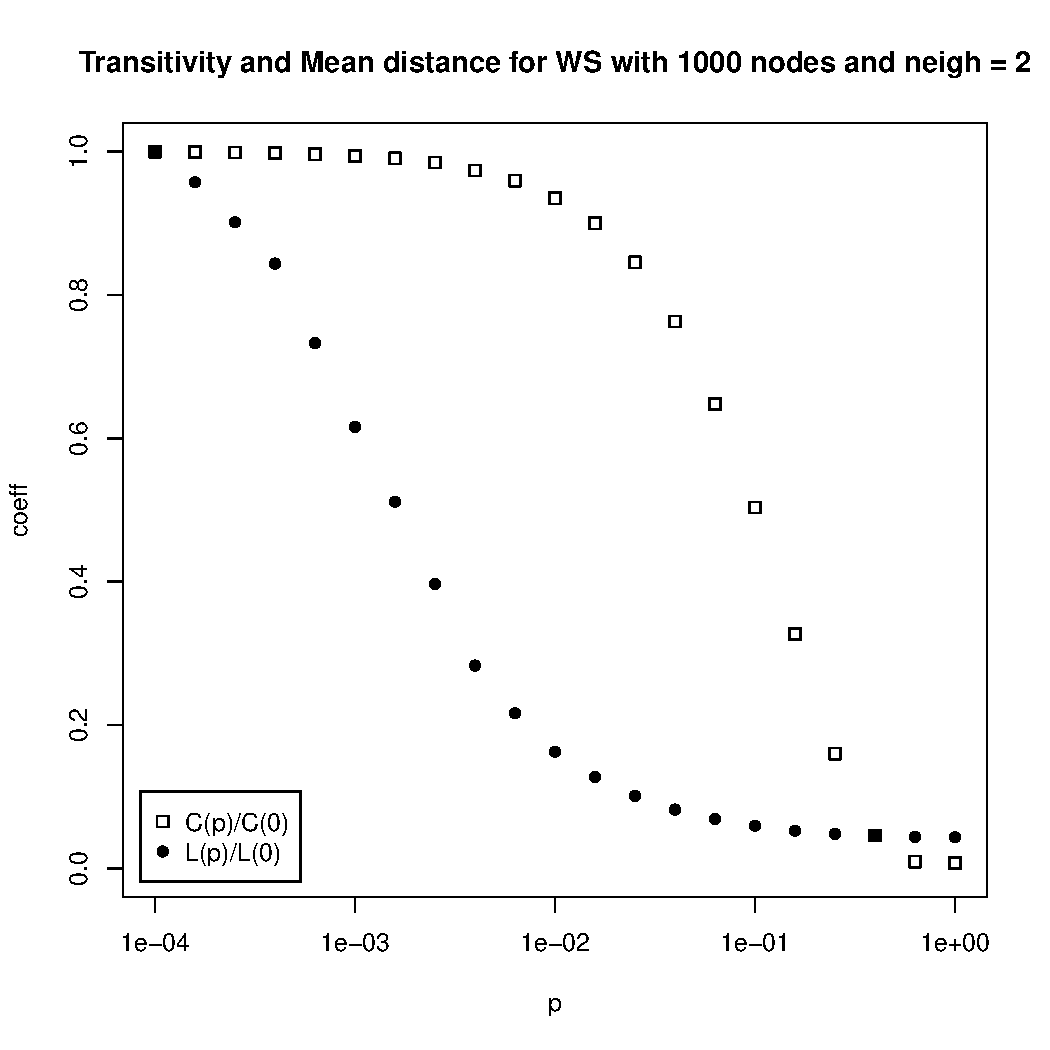
\includegraphics[width=0.66\textwidth]{figures/WS_neigh_2.pdf}
    \caption{Evolution of Clustering Coefficient $L(p)$ and the average shortest-path $C(p)$}
    \label{fig:ws}
\end{figure}

During our experimental investigations aimed at determining suitable mean degree values, an intriguing anomaly emerged, as depicted in Figure \ref{fig:ws_high_neigh}. Contrary to expectations, the Clustering Coefficient did not approach zero even at significantly high values of $p$. This behavior can be attributed to the inherent structure of the random graph model, where the presence of local clustering is preserved even at higher $p$ values. Additionally, our choice of normalization with respect to $L(0)$ contributes to this outcome, ensuring that the clustering coefficient doesn't deviate significantly from $L(0)$ due to the graph's elevated mean degree.

\begin{figure}
    \centering
    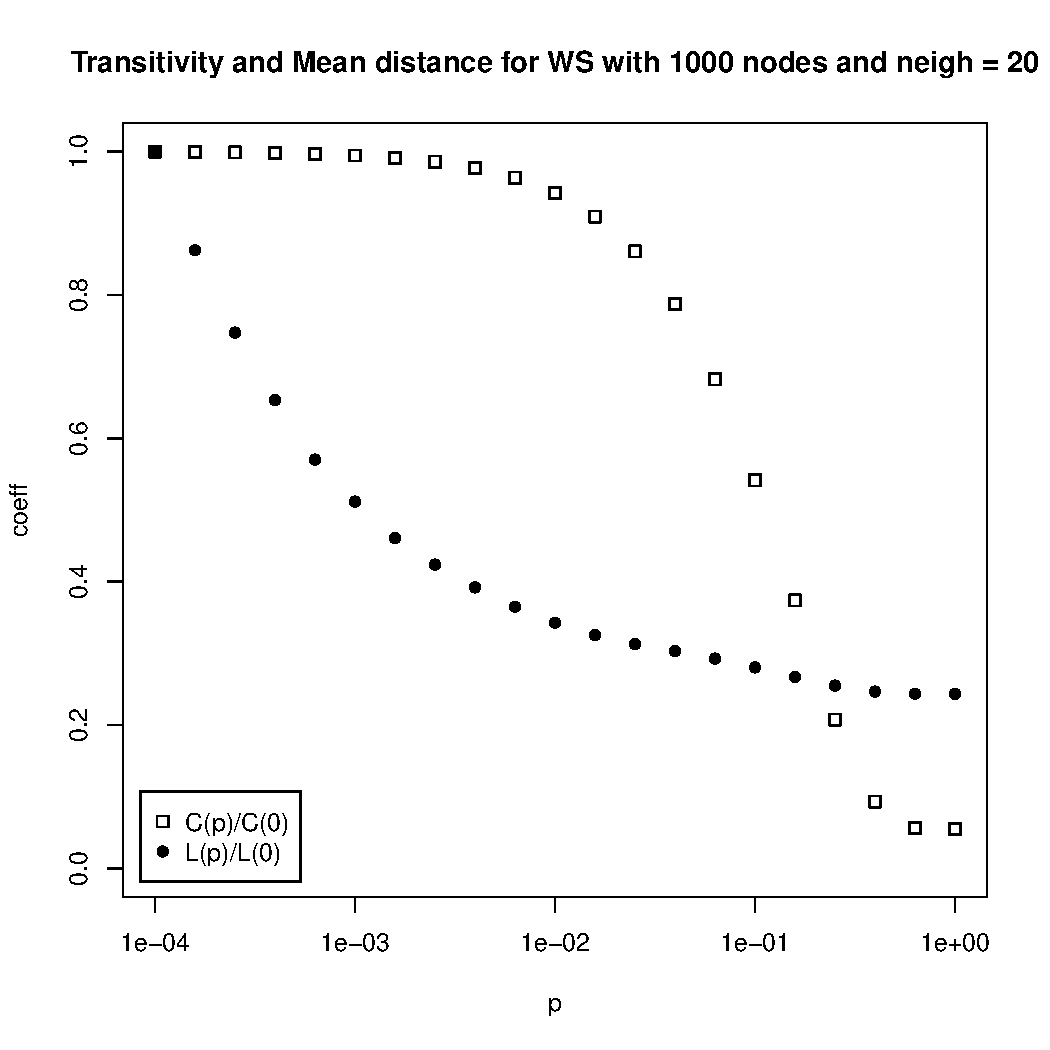
\includegraphics[width=0.66\textwidth]{figures/WS_neigh_20.pdf}
    \caption{Evolution of Clustering Coefficient $L(p)$ and the average shortest-path $C(p)$}
    \label{fig:ws_high_neigh}
\end{figure}
\chapter{Erdös-Rényi model}
\label{cha: Erdös-Rényi model}
The Erdös-Rényi model is used to generate random graphs. It is a model that allows for the generation of graphs with a small diameter. This is a property that is also found in real networks. Contrary to real networks or the other models discussed in the lectures, it does not posses the property of high clustering nor it is scale-free. To plot the average shortest-path as a function of the network size the two variables for the Erdös-Rényi model G(n,p) have to be chosen accordingly. The graph from the task sheet uses zero to one million nodes and an unknown \textit{p} value. To calculate a suitable \textit{p} value that allows for a connected graph we use the following formulas from \cite{Erdos1984OnTE}.
\begin{itemize}
    \item If $ \,p < \frac{(1-\epsilon) \, ln \, n}{n} \,$ then a graph in G(n,p) will almost surely contain isolated vertices, and thus be disconnected.
    \item If $ \,p > \frac{(1-\epsilon) \, ln \, n}{n} \,$ then a graph in G(n,p) will almost surely be connected.
\end{itemize}
Because of insufficient hardware we had to reduce the maximum number of nodes \textit{n} that are considered to one hundred thousand instead of one million. Furthermore in the case that the graph is not fully connected we consider only the largest fully connected sub-graph. The graph from the task can not be recreated with a constant \textit{p} value for all values of \textit{n}. For example using a \textit{p} value of 0.1 for all values of \textit{n} results in the graph that can be seen in \ref{fig:ER Model with p = 0.1}.
We believe that using a rather large \textit{p} value of 0.1 leads to the creation of large central components in the graph once the \textit{n} value is adequately large. These central components lead to small shortest paths on average.
Therefore the value of \textit{p} has to be chosen in accordance of the value of \textit{n} to recreate the graph from the assignment. We have used the p value of $\,2\,ln(n)/n\,$, this is also recommended by the relevant literature to this topic. The resulting graph can be seen in \ref{fig:ER Model with dynamic P}. This graph shows that the average shortest path increases sharply with with the amount of nodes before reaching an stable value.
\begin{figure}
    \centering
    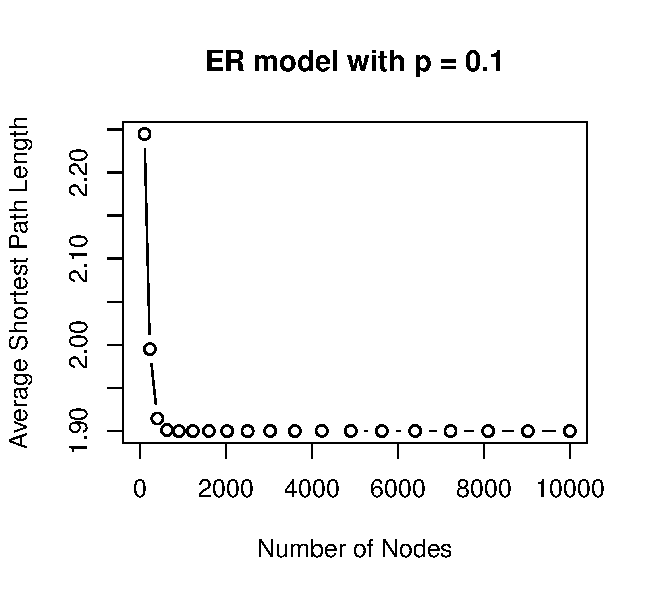
\includegraphics[width=0.66\textwidth]{figures/ER model with p = 0.1.pdf}
    \caption{ER model with a static \textit{p} of 0.1 and a maximal \textit{n} of 10000}
    \label{fig:ER Model with p = 0.1}
\end{figure}
\begin{figure}
    \centering
    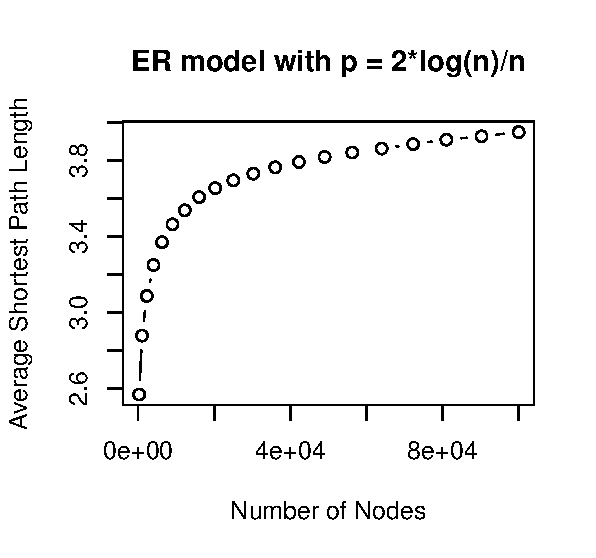
\includegraphics[width=0.66\textwidth]{figures/ermodelp2lognn100000.pdf}
    \caption{ER model with a dynamic \textit{p} of $\,2\,ln(n)/n\,$ and a maximal \textit{n} of 100000}
    \label{fig:ER Model with dynamic P}
\end{figure}

\bibliographystyle{plain}
\bibliography{seminar-ref}

\end{document}
